\documentclass[11pt,a4paper]{article}
\usepackage[T1]{fontenc}
\usepackage[utf8]{inputenc}
\usepackage{lmodern}
\usepackage[a4paper,margin=22mm]{geometry}
\usepackage{graphicx}
\usepackage{microtype}
\usepackage[numbers,sort&compress]{natbib}
\usepackage{caption}
\usepackage[hidelinks,unicode]{hyperref}
\hypersetup{pdftitle={Cellular organization of inflammatory transcription in the mouse cochlea after acoustic trauma},pdfauthor={Dengxiang Yang}}
\urlstyle{same}
\newcommand{\doi}[1]{\url{https://doi.org/#1}}
\linespread{1.10}
\setlength{\parindent}{1.2em}
\setlength{\parskip}{3pt}
\setlength{\emergencystretch}{2em}
\clubpenalty=10000
\widowpenalty=10000
\displaywidowpenalty=10000
\captionsetup{font=small,labelfont=bf,justification=justified,singlelinecheck=false}
\renewcommand{\refname}{References}
\makeatletter
\setlength{\@fptop}{0pt}
\setlength{\@fpsep}{14pt}
\setlength{\@fpbot}{0pt plus 1fil}
\makeatother

\renewcommand{\thefigure}{S\arabic{figure}}
\renewcommand{\figurename}{Supplementary Figure}
\begin{document}
\captionsetup{font=small}
\begin{center}
{\large\bfseries Supplementary Information}\par\vspace{3pt}
{\normalsize\bfseries Cellular organization of inflammatory transcription in the mouse cochlea after acoustic trauma}\par\vspace{3pt}
{\small Dengxiang Yang\par Southern University of Science and Technology, Shenzhen, China\par\href{mailto:12412602@mail.sustech.edu.cn}{12412602@mail.sustech.edu.cn}}
\end{center}
\noindent\begin{minipage}{\linewidth}
\centering
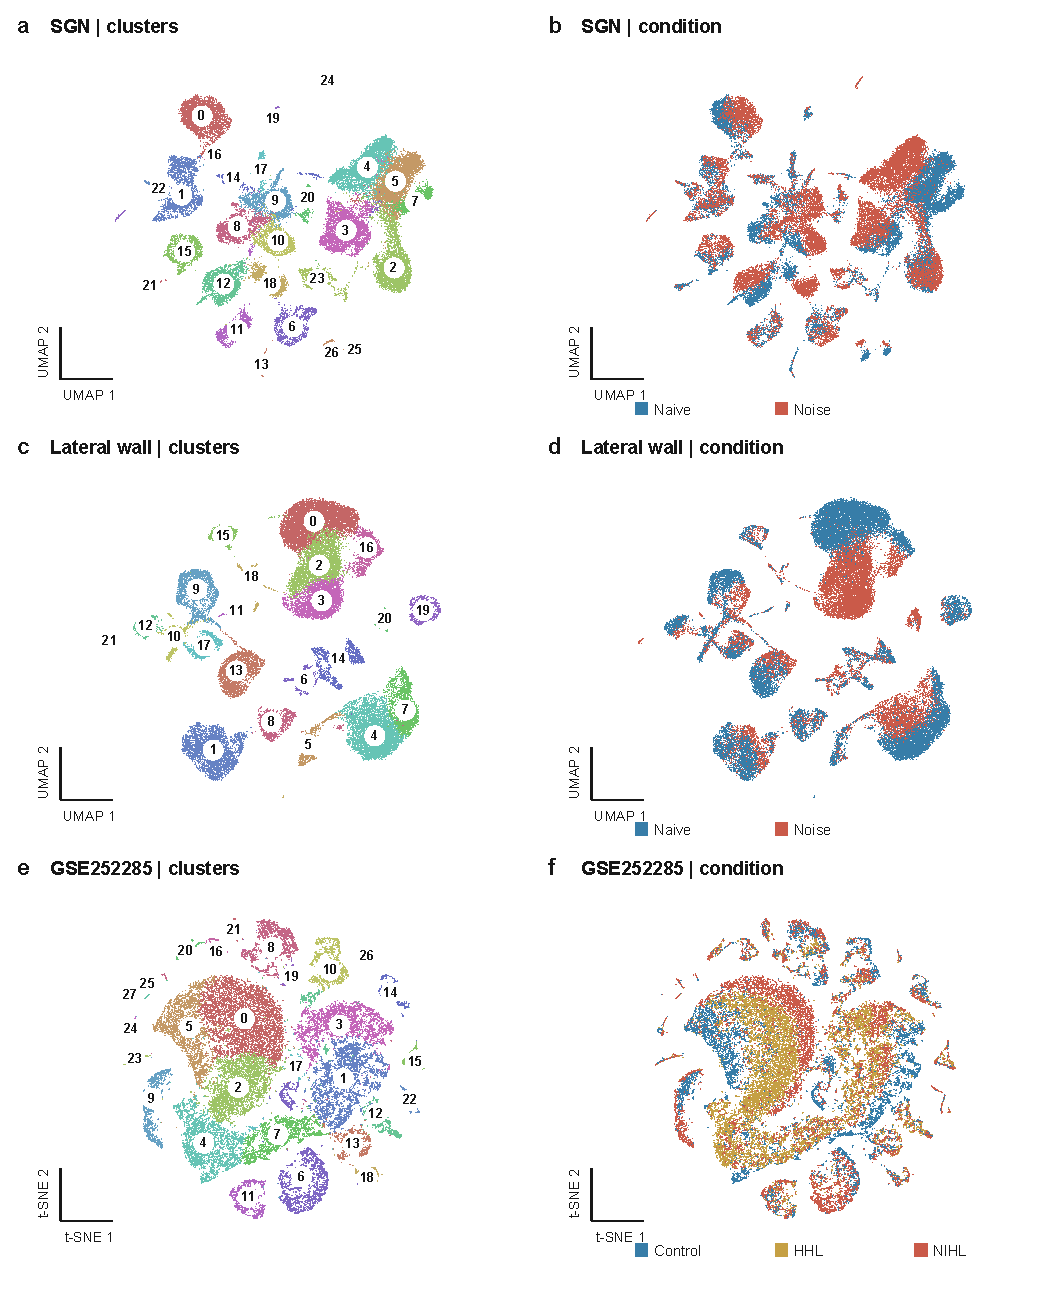
\includegraphics[width=\linewidth,height=0.68\textheight,keepaspectratio]{figures/FigureS1_cluster_and_condition_maps.pdf}
\captionof{figure}{\textbf{Cluster structure and condition distributions in the cell embeddings.} (a,b) Spiral-ganglion-region UMAP projections coloured by the 27 Leiden clusters or experimental condition. (c,d) Lateral-wall UMAP projections coloured by the 22 Leiden clusters or condition. (e,f) GSE252285 t-SNE projections coloured by the selected 28 clusters or resolved library condition. Cluster numbers identify the stored clustering solutions. All panels display the same retained cells and coordinates as Figure 1. Naive and Noise denote the GSE168041 groups; Control, HHL and NIHL denote the three GSE252285 libraries.}
\label{fig:S1}
\end{minipage}
\clearpage
\begin{figure}[p]
\centering
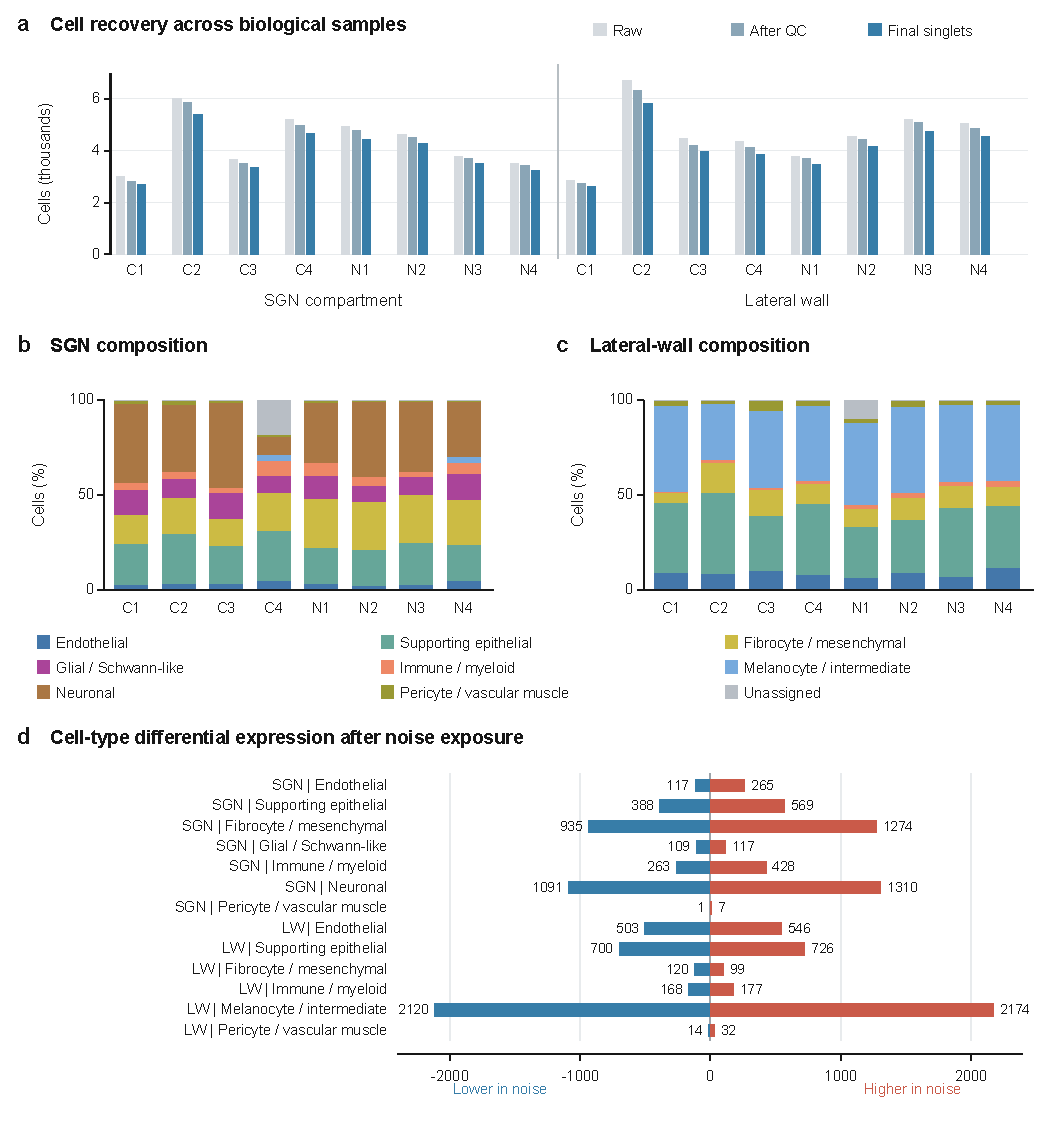
\includegraphics[width=\linewidth,height=0.72\textheight,keepaspectratio]{figures/FigureS2_cell_type_landscape.pdf}
\caption{\textbf{Cellular composition and differential expression across cochlear compartments.} (a) Raw, quality-controlled and final singlet counts for each GSE168041 sample. C1--C4 denote naive samples and N1--N4 denote noise-exposed samples within each compartment. (b,c) Broad cell-type fractions within each SGN and lateral-wall sample, including unassigned cells. (d) Numbers of genes with Benjamini--Hochberg FDR \(<\) 0.05 in sample-level pseudobulk contrasts of noise versus naive tissue. Blue and red bars indicate lower and higher expression after noise exposure, respectively. Each cell-type comparison used four naive and four noise-exposed samples. LW, lateral wall; SGN, spiral ganglion region. The counts in panel d use the complete tested gene sets without an additional fold-change cutoff.}
\label{fig:S2}
\end{figure}
\clearpage
\begin{figure}[p]
\centering
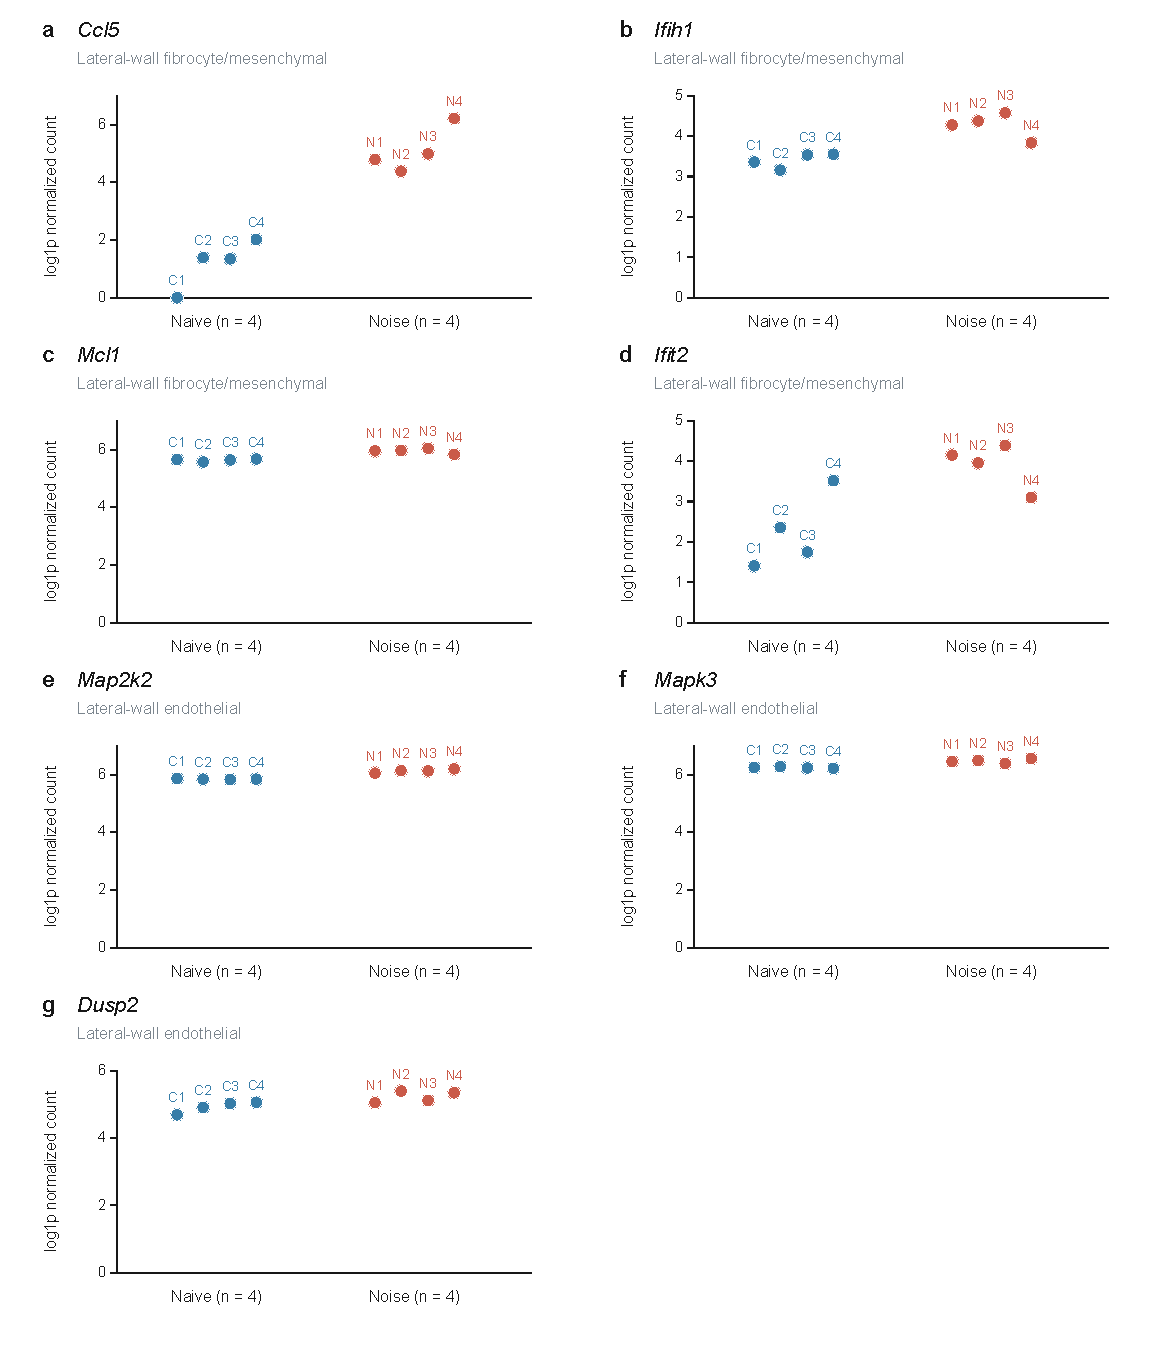
\includegraphics[width=\linewidth,height=0.78\textheight,keepaspectratio]{figures/FigureS3_sample_gene_expression.pdf}
\caption{\textbf{Representative gene expression in individual biological samples.} Points show log1p-transformed normalized counts from the full-sample GSE168041 pseudobulk models. \textit{Ccl5}, \textit{Ifih1}, \textit{Mcl1} and \textit{Ifit2} are displayed in lateral-wall fibrocyte/mesenchymal samples; \textit{Map2k2}, \textit{Mapk3} and \textit{Dusp2} are displayed in lateral-wall endothelial samples. Each condition contains four biological samples. C1--C4 denote naive samples and N1--N4 denote noise-exposed samples. Counts use the full-model size factors. GEO sample identifiers and untransformed normalized counts accompany the source data.}
\label{fig:S3}
\end{figure}
\clearpage
\begin{figure}[p]
\centering
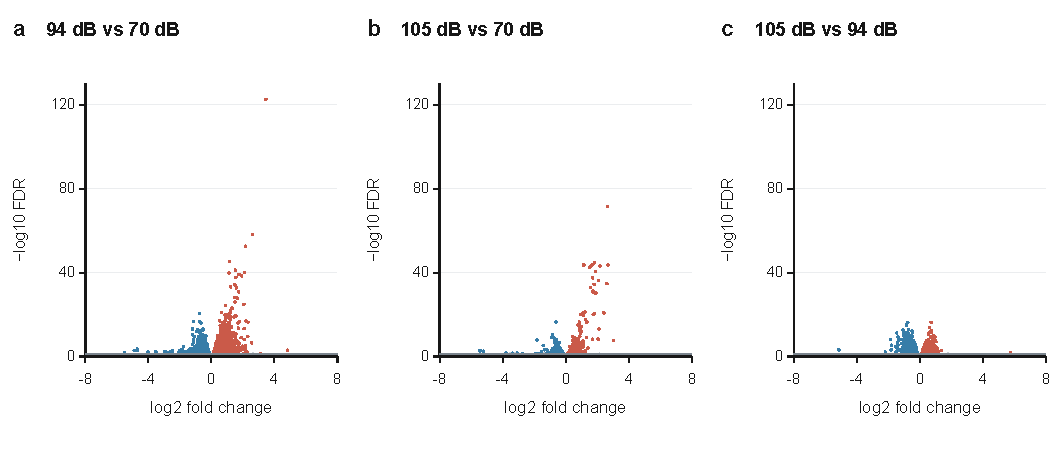
\includegraphics[width=\linewidth,height=0.38\textheight,keepaspectratio]{figures/FigureS4_bulk_volcanoes.pdf}
\captionsetup{font=normalsize}
\caption{\textbf{Gene-level differential expression across whole-cochlea exposure comparisons.} Volcano plots show the raw-count DESeq2 \(\log_2\) fold changes and \(-\log_{10}\) adjusted P values for 94 versus 70 dB, 105 versus 70 dB and 105 versus 94 dB. Blue and red points denote FDR \(<\) 0.05 with negative and positive fold changes, respectively; grey points denote other genes with finite adjusted P values. The dashed line indicates FDR = 0.05. For display, \(\log_2\) fold changes are clipped at \(\pm\)8 and \(-\log_{10}\) FDR at 130. Genes lacking a finite adjusted P value are omitted from the display and retained in the source tables. The respective display-omission counts were 791, 3,077 and 3,837 genes.}
\label{fig:S4}
\end{figure}
\clearpage
\begin{figure}[p]
\centering
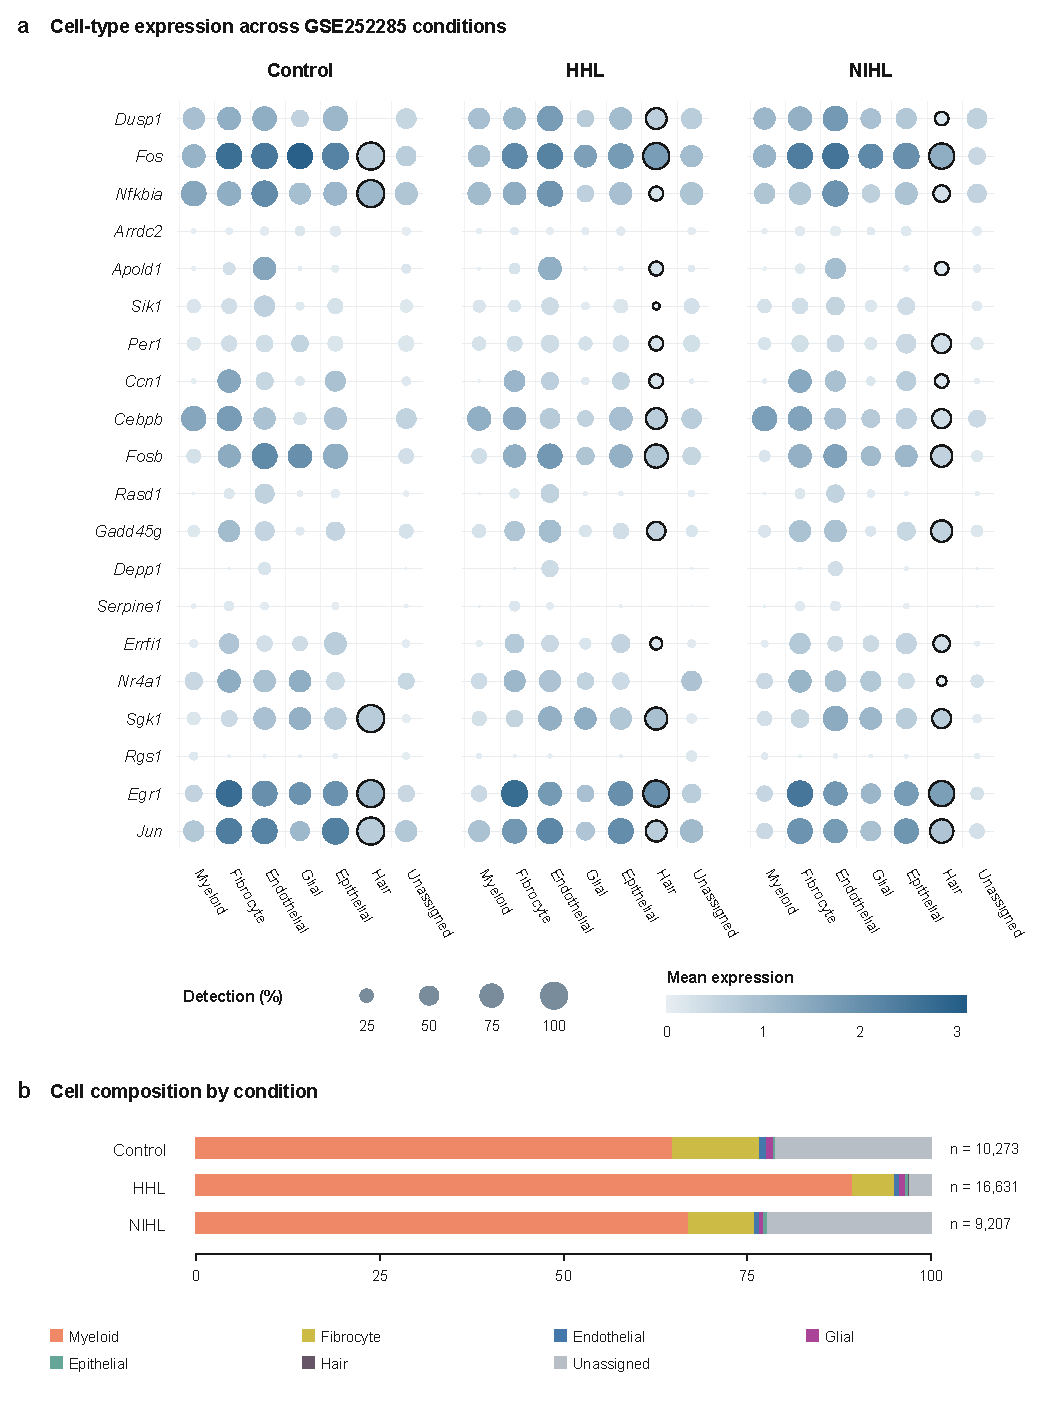
\includegraphics[width=\linewidth,height=0.84\textheight,keepaspectratio]{figures/FigureS5_all_twenty_genes.pdf}
\caption{\textbf{Condition-resolved expression of the complete twenty-gene panel.} All twenty genes in the panel are shown using the same cell-type labels, dot-area encoding and common expression scale as Figure 5. Outlined dots denote cell groups with fewer than 20 cells. Condition-level distributions summarize cells within each library. HHL, hidden hearing loss; NIHL, noise-induced hearing loss.}
\label{fig:S5}
\end{figure}
\clearpage
\begin{figure}[p]
\centering
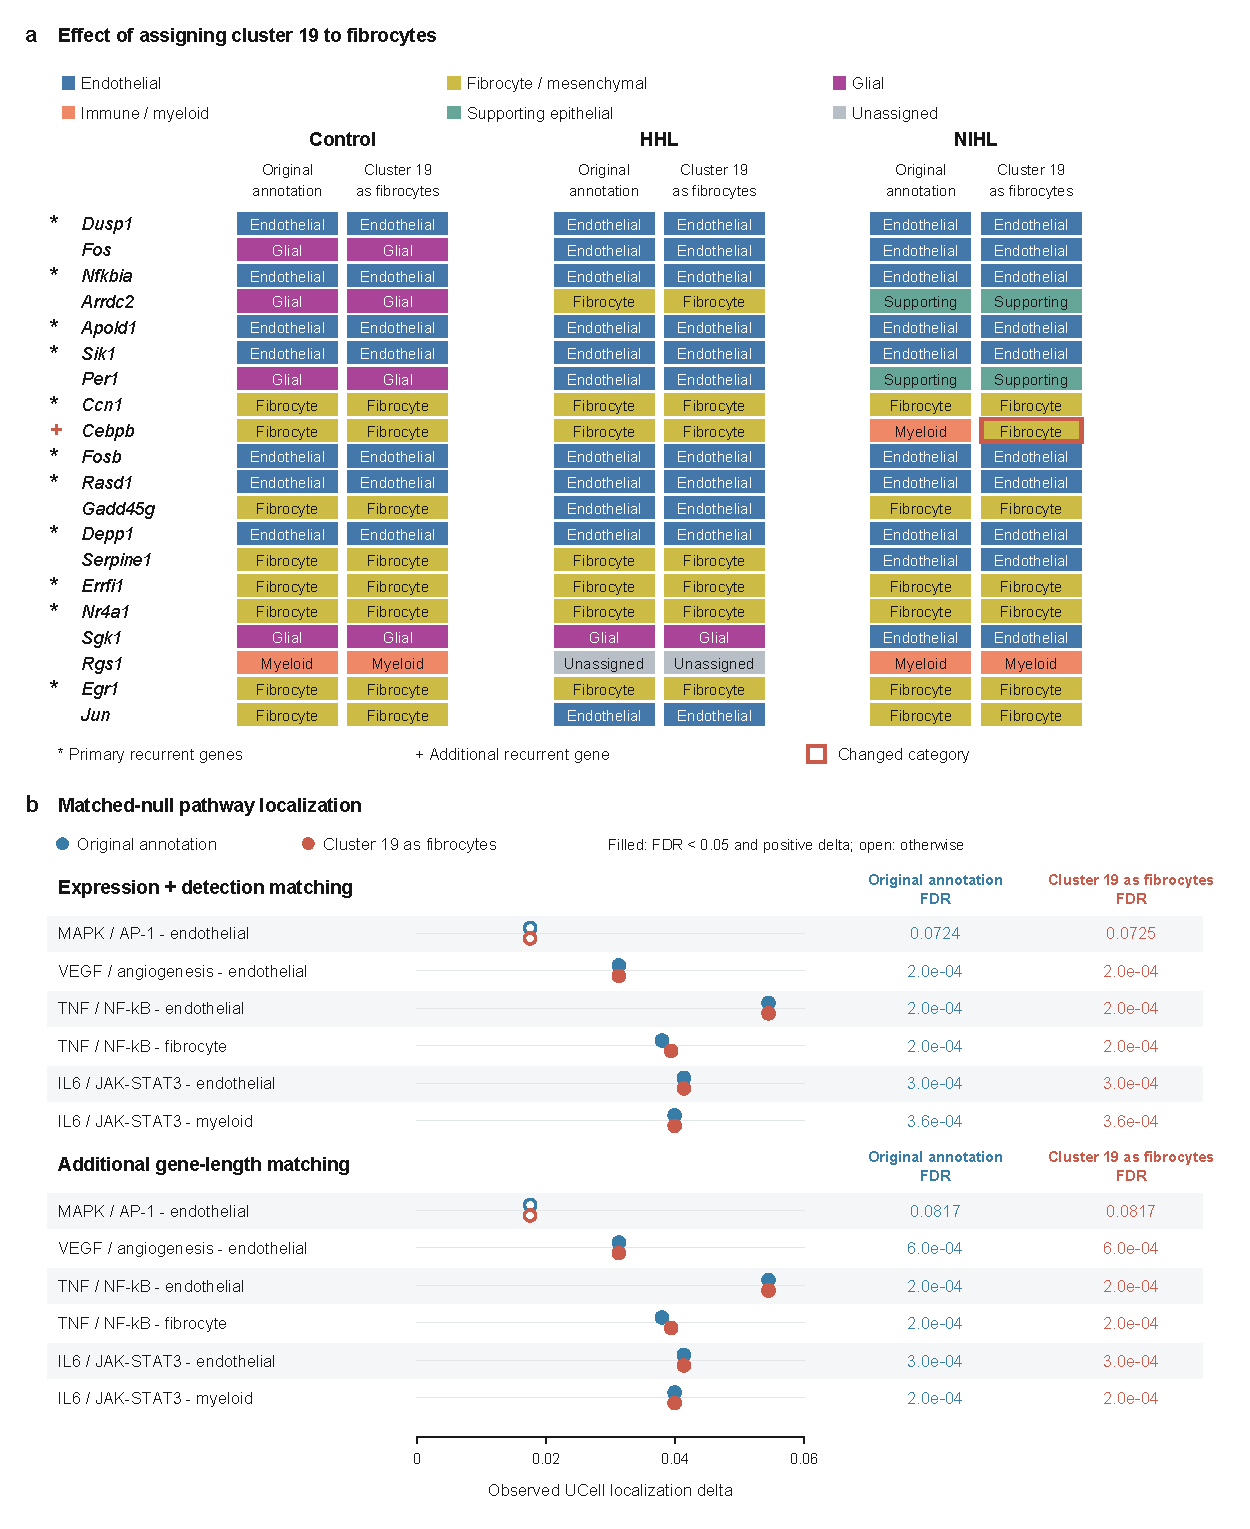
\includegraphics[width=\linewidth,height=0.78\textheight,keepaspectratio]{figures/FigureS6_annotation_sensitivity.pdf}
\caption{\textbf{Gene and pathway localization after reassignment of cluster 19.} (a) Highest-mean-expression broad categories for all twenty panel genes in Control, HHL and NIHL under the primary annotation and reassignment of the 319 cluster 19 cells to fibrocyte/mesenchymal. Asterisks mark the eleven recurrent primary assignments, all retained. \textit{Cebpb} additionally becomes recurrent (+); the red outline identifies its changed NIHL assignment. (b) All six UCell-guided localization comparisons under both annotations, using expression--detection matching and additional gene-length matching. Points show the target-category median UCell score minus the median of the other five resolved-category medians. The two annotations use the same frozen inputs and random signatures, with 10,000 random sets per program and matching scheme. One-sided empirical P values were BH-adjusted across the six comparisons within each scheme. Filled points denote positive statistics with FDR \(<\) 0.05; hollow points denote the remaining results.}
\label{fig:S6}
\end{figure}
\clearpage
\begin{figure}[p]
\centering
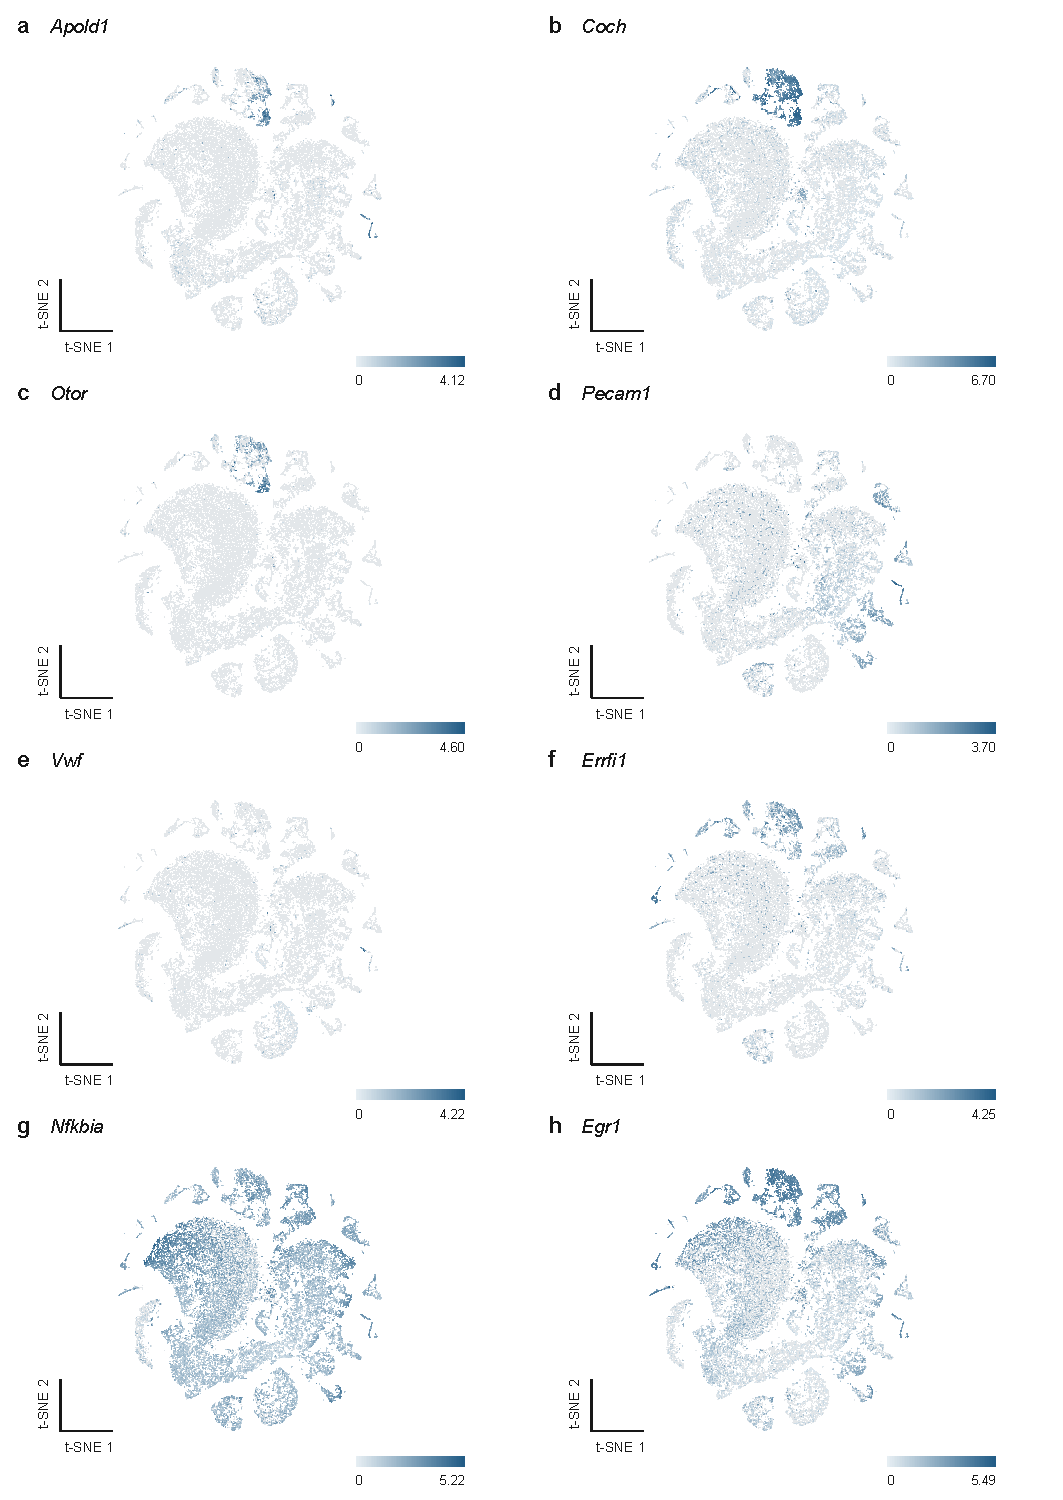
\includegraphics[width=\linewidth,height=0.82\textheight,keepaspectratio]{figures/FigureS7_gene_feature_maps.pdf}
\caption{\textbf{Gene-expression distributions in the GSE252285 t-SNE space.} The eight panels display \textit{Apold1}, \textit{Coch}, \textit{Otor}, \textit{Pecam1}, \textit{Vwf}, \textit{Errfi1}, \textit{Nfkbia} and \textit{Egr1} across all 36,111 cells. Grey points have zero expression; blue intensity represents the Seurat log-normalized RNA value. Each panel's colour scale spans zero to its displayed maximum. Coordinates and cell inclusion match Figure 1c.}
\label{fig:S7}
\end{figure}
\clearpage
\begin{figure}[p]
\centering
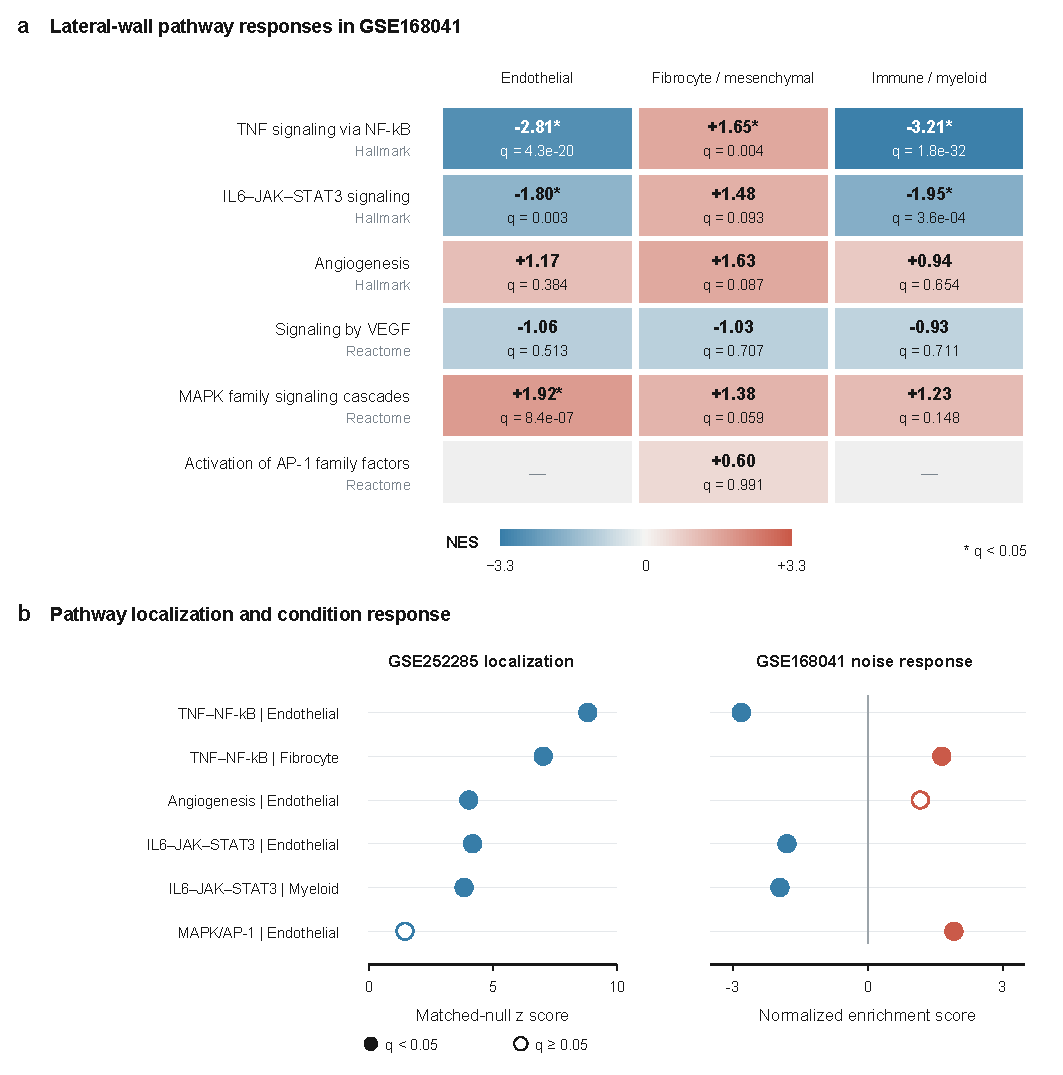
\includegraphics[width=\linewidth,height=0.70\textheight,keepaspectratio]{figures/FigureS8_localization_and_cell_state.pdf}
\caption{\textbf{Matched-null localization tests and corresponding cell-state estimates.} (a) Normalized enrichment scores (NES) and FDR values for the six focused Hallmark and Reactome gene sets in lateral-wall endothelial, fibrocyte/\allowbreak{}mesenchymal and immune/\allowbreak{}myeloid cells in GSE168041. Positive NES denotes enrichment toward noise-exposed samples. Asterisks identify FDR \(<\) 0.05. Grey cells with a dash mark gene sets outside the eligible size range. Each pseudobulk contrast used four samples per condition. (b) The six UCell-guided follow-up localization comparisons in GSE252285 are displayed beside the corresponding GSE168041 condition-response estimates. Left, z scores relative to 10,000 expression- and detection-matched random gene sets; right, NES from sample-level differential-expression rankings. Filled points denote FDR \(<\) 0.05 within the corresponding analysis. The sixth row pairs the MAPK/\allowbreak{}AP-1 localization signature with the Reactome MAPK family signaling cascades set; these are distinct gene sets. Localization compares signature scores across cell types; condition response compares noise-exposed and unexposed samples. Hallmark angiogenesis and Reactome VEGF signaling are displayed separately in panel a.}
\label{fig:S8}
\end{figure}
\clearpage
\section*{Supplementary Table S1. Selection of genes and pathway comparisons}
\noindent\begin{tabular}{p{0.21\linewidth}p{0.70\linewidth}}
\raggedright\textbf{Analysis set} & \raggedright\textbf{Selection and use} \tabularnewline
\hline
\raggedright Twenty candidate genes & \raggedright Author-selected exploratory panel retained across the three GSE252285 libraries. Cell categories were ranked by mean normalized expression, using detection fraction to resolve ties. \tabularnewline[7pt]
\raggedright Nine bulk pathways & \raggedright A targeted panel covering inflammatory and cytokine signaling, proteostasis, oxidative stress and apoptosis. The same nine definitions were applied to all three GSE160639 contrasts; BH adjustment covered 27 pathway--contrast combinations. \tabularnewline[7pt]
\raggedright Six UCell programs & \raggedright Mouse MSigDB sets or deterministic unions representing MAPK/AP-1, TNF--NF-\(\kappa\)B, IL6--JAK--STAT3, VEGF/angiogenesis, MYC targets and E2F targets. Scores were summarized across broad cell categories. \tabularnewline[7pt]
\raggedright Six follow-up comparisons & \raggedright Initial UCell profiles guided endothelial MAPK/AP-1 and VEGF/angiogenesis; endothelial and fibrocyte/mesenchymal TNF--NF-\(\kappa\)B; and endothelial and immune/myeloid IL6--JAK--STAT3 comparisons. Empirical matched-gene-set FDRs refer to this six-comparison follow-up family, separately for each matching scheme. \tabularnewline
\hline
\end{tabular}
\par\vspace{14pt}\noindent Exact gene memberships, target categories and selection-source records accompany Supplementary Table S1 in the source data.
\end{document}
